\section{Escenarios}
Para comprobar el correcto funcionamiento de todo lo implementado se han creado varios escenarios. Por un lado se han utilizado tres escenarios proporcionados por el profesor, que están en la carpeta \textit{\_escenasEvaluacion} donde se ha utilizado uno para comprobar que el PathFindingLrta funciona correctamente, por otro lado el escenario creado para wall Avoidance con paredes y esquinas de varios ángulos, donde tal y como se comentará en la exposición en las esquinas hay veces donde a los personajes les cuesta salir. Por último el escenario de formaciones que se utiliza para comprobar que las formaciones se hacen correctamente y en el caso de formar al lado de esquinas o paredes, que los personajes no las atraviesan.\\

En cuanto a escenarios creados por nosotros, tenemos dos escenarios para probar steerings:
\begin{itemize}
    \item SteeringsBasicos: este escenario tendrá un personaje por cada steering básico implementado y permitirá manejar el player para poder ver cómo se adapta cada NPC a la posición del player según el script que contenga.
    \item SteeringsDelegados: Este escenario es igual que el anterior nada más que tendrá un NPC por cada Steering delegado.
\end{itemize}
El escenario \textit{WallAvoidance} consta de una pared y un NPC y un player, y ha servido para probar el comportamiento de wallAvoidance, aunque el de evaluación ha sido el que más se ha utilizado ya que tenía esquinas de distintos ángulos que permiten ver en mayor profundidad cómo se comporta este. \\

Por último tenemos la escena de \textit{PathFollow} que consta de un camino creado a base de waypoints donde se verá cómo de bien funciona dicho script.
\section{Steerings}

En este apartado veremos como implementar un sistema de steerings para un conjunto de escenas controlado. También existirán opciones como hacer formaciones.

Un sistema de steering es un sistema encargado de calcular un movimiento de respuesta a los agentes en función de la información que tienen sobre el entorno que les rodea. Los steerings se pueden combinar entre ellos de forma que obtengamos comportamientos distintos. Por ejemplo, podemos hacer que un agente persiga a otro, pero a la vez trate de evitar obstáculos.

En nuestro caso se han implementado tanto steerings básicos acelerados como steerings delegados. Estos tipos de steering heredan de la clase \texttt{SteeringBehavior}, que contiene los elementos básicos que deben tener.

\begin{itemize}
    \item Atributos:
    \begin{itemize}
        \item \texttt{nameSteering}: el nombre del steering.
        \item \texttt{target}: representa al agente sobre el que se toman las referencias, como distancia hasta él o diferencia en orientación.
        \item \texttt{weight}: el peso que tiene este steering a la hora de combinarse con otros (se usa en los árbitros ponderados). 
    \end{itemize}
    \item El método \texttt{GetSteering(Agent agent)} que devolverá el steering calculado en cuestión.
\end{itemize}

Para modelizar el comportamiento que devuelto un steering behavior se usa una estructura \texttt{Steering}, que consta de dos componentes.

\begin{itemize}
    \item \texttt{angular}: es la componente que modifica el comportamiento del agente desde el punto de vista de la orientación. Generalmente lo tomamos como aceleración angular, pero podría representar otra magnitud dependiendo del comportamiento que busquemos. Es un valor escalar.
    \item \texttt{linear}: es la componente que modifica el comportamiento del agente en cuanto a la posición. Normalmente representa la aceleración lineal del personaje, pero puede representar una velocidad también u otra magnitud a voluntad. Es una componente vectorial.
\end{itemize}

\subsection{Steerings básicos}

Los Steerings básicos acelerados que se han implementado son: Seek, Flee, Arrive, Align, Anti-Align y Velocity Matching. Veremos uno por uno cómo se han implementado y las particularidades que puedan tener cada uno de ellos.

\subsubsection{Seek}

Este steering calcula un movimiento en línea recta desde la posición del agente hasta la posición del agente objetivo, representado por la variable \texttt{target}.

Lo primero a realizar será calcular la distancia entre los agentes y en el caso de que sea menor que el radio interior del objetivo  frenamos.

\lstinputlisting[linerange=22-30, firstnumber=22]{\ScriptsPath/Steering/Basic/Seek.cs}

En el caso de que el objetivo esté a una distancia mayor que el radio interior del agente se usa la máxima aceleración en la dirección del desplazamiento.

\lstinputlisting[linerange=32-38, firstnumber=32]{\ScriptsPath/Steering/Basic/Seek.cs}


\subsubsection{Flee}

El comportamiento de este steering es contrario al steering anterior. El agente que implemente este steering se moverá en dirección opuesta a la del agente objetivo, ``huyendo'' de él.

\lstinputlisting[linerange=22-27, firstnumber=22]{\ScriptsPath/Steering/Basic/Flee.cs}


\subsubsection{Arrive}

Este steering tiene un comportamiento similar al del Seek, calcula un movimiento en línea recta desde un agente a la posición de otro. La diferencia está en que este steering se tienen en cuenta dos radios en la posición objetivo, se muestra en la Fig. \ref{fig:arrive}. 

\begin{figure}[H]
    \centering
    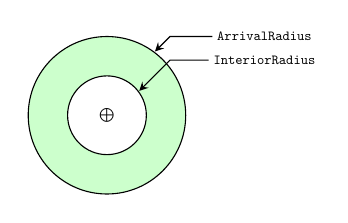
\begin{tikzpicture}
        \node[circle, minimum size=2cm, draw, fill=green!20] (1) {};
        \node[circle, minimum size=1cm, draw, fill=white] (2) {};
        \node[scale=0.5] (3) {$\bigoplus$};
        \node[scale=0.5] (4) at (2, 1) {\texttt{ArrivalRadius}};
        \node[scale=0.5] (5) at (2, 0.7) {\texttt{InteriorRadius}};
        
        \draw[-stealth] (4) -- (0.8, 1) -- (0.61, 0.81);
        \draw[-stealth] (5) -- (0.8, 0.7) -- (0.41, 0.31);
    \end{tikzpicture}
    \caption{Esquema del steering Arrive}
    \label{fig:arrive}
\end{figure}

Cuando estamos fuera de ambos radios se aplicará una velocidad máxima, con el objetivo de llegar rápido al punto. Si estamos en la región entre ambos radios se aplica una velocidad máxima escalada en función de la distancia entre los agentes.

\lstinputlisting[linerange=38-55, firstnumber=38]{\ScriptsPath/Steering/Basic/Arrive.cs}

En caso de que los agentes estén lo suficientemente cerca, es decir, dentro de la región del radio interior, se frena al agente.

\lstinputlisting[linerange=31-36, firstnumber=31]{\ScriptsPath/Steering/Basic/Arrive.cs}


Por último comprobamos sí la aceleración calculada es superior a la máxima aceleración del personaje, y en caso de ser superior la acotamos. 

\lstinputlisting[linerange=57-64, firstnumber=57]{\ScriptsPath/Steering/Basic/Arrive.cs}


\subsubsection{Align}

Este steering hace que un agente mire en la misma dirección que otro, sin prestar atención a ningún aspecto de la posición del agente. Para hacer esto usa la diferencia entre las orientaciones de los agentes.

En este caso en vez de calcular la distancia, se calcula la diferencia entre orientaciones.

\lstinputlisting[linerange=23-29, firstnumber=23]{\ScriptsPath/Steering/Basic/Align.cs}

De forma similar a como se actuaba el Arrive en este caso se comprueba si el desalianeamiento es mayor que el ángulo exterior para usar la rotación máxima.

\lstinputlisting[linerange=38-47, firstnumber=38]{\ScriptsPath/Steering/Basic/Align.cs}

El resto del código es igual que el visto en Arrive (cambiando \texttt{steer.linear} por \texttt{steer.angular}), comprobando si la aceleracion es demasiado grande, en caso de que si se establecerá al máximo.


\subsubsection{Anti-Align}

Este steering consiste en realizar el movimiento contrario que el steering anterior. En este caso el personaje tiene que tener una rotación opuesta a la del objetivo, es por esto que el único cambio a realizar sobre el align será sumar \SI[parse-numbers=false]{\pi}{\radian} (\SI{180}{\degree}) a su orientación y alinear para este valor.

\lstinputlisting[linerange=24-28, firstnumber=24]{\ScriptsPath/Steering/Basic/AntiAlign.cs}


\subsubsection{Velocity Matching}

En este steering el objetivo es que el agente replique el movimiento de otro. Para realizar esto sólo nos fijaremos en la velocidad del otro agente, ya que esta al ser vectorial, también tiene la dirección del movimiento.

\lstinputlisting[linerange=23-32, firstnumber=23]{\ScriptsPath/Steering/Basic/VelocityMatching.cs}



